\documentclass{article}
\usepackage{amsmath}
\usepackage{amssymb}
\usepackage{fancyhdr}
\usepackage{hyperref}
\usepackage{tikz}
\usepackage{geometry}

\geometry{letterpaper, portrait, margin=0.5in}
\pagestyle{fancy}

\fancyhf{} % clear all header fields
\renewcommand{\headrulewidth}{0pt}
\fancyfoot[LE,RO]{\thepage}           % page number in "outer" position of footer line
\fancyfoot[RE,LO]{\copyright\;aquarc 2024. \href{https://aquarc.org}{\underline{aquarc.org}}} % other info in "inner" position of footer line

\title{SAT Math Equations}

\begin{document}

\fontsize{14}{16}\selectfont

\maketitle

\tableofcontents
\pagebreak

\section{Quadratics}

A quadratic is a function in the form
$$
f(x) = ax^2 + bx + c
$$
Where ${\{a, b, c\}} \in \mathbb{R}$.

Or in the vertex form:
$$
f(x) = a(x-h)^2 + k
$$
Where ${\{a, h, k\}} \in \mathbb{R}$

Or in the roots form:
$$
f(x) = a(x-r_1)(x-r_2)
$$
Where ${\{a, r_1, r_2\}} \in \mathbb{R}$

\subsection{FOIL}
FOIL stands for First Outer Inner Last. Meaning, when you have
$$
f(x)=(a_1x-r_1)(a_2x-r_2)
$$

You get:
$$
a_1a_2x^2-a_1r_2x-a_2r_1x+r_1r_2 =a_1a_2x^2-(a_1r_1+a_2r_2)x+(r_1r_2)
$$

\subsection{Quadratic Formula}

\subsubsection{Derivation}

$$
ax^2+bx+c=0 \Longrightarrow 
ax^2+bx=-c \Longrightarrow 
\frac{1}{a}ax^2+\frac{b}{a}x=-\frac{c}{a} 
\Longrightarrow
x^2+\frac{b}{a}x=-\frac{c}{a} 
$$
Complete the square:
$$
x^2+\frac{b}{a}x+\frac{b^2}{4a^2}=-\frac{c}{a} + \frac{b^2}{4a^2} \Longrightarrow
(x+\frac{b}{2a})^2=-\frac{4ac}{4a^2} + \frac{b^2}{4a^2} \Longrightarrow
(x+\frac{b}{2a})^2=\frac{b^2-4ac}{4a^2} 
$$
$$
\Longrightarrow
\sqrt{(x+\frac{b}{2a})^2}=\frac{\pm\sqrt{b^2-4ac}}{2a} \Longrightarrow
x=\frac{-b\pm\sqrt{b^2-4ac}}{2a}
$$

\subsubsection{Alternatives}

In some scenarios it may be easier to use systems of equations.

Given a quadratic in the form:
$$
ax^2+bx+c=0
$$
We want to find $r_1$ and $r_2$ such that:
$$
r_1+r_2=b \quad r_1r_2=c
$$

You can easily subsitute around until you get the answer.
If $a \neq 1$ then it is difficult to use this formula.

% todo: it is possible but how 

\subsection{Discriminant}

The discriminant tells you whether a quadratic is going to have real or imaginary roots. \\
If we look at the quadratic formula for earlier:

$$
x=\frac{-b\pm\sqrt{b^2-4ac}}{2a}
$$
The term $\pm\sqrt{b^2-4ac}$ denotes the possibility of two solutions or one solution or none. \\
If $\sqrt{b^2-4ac} > 0$ then the $\pm$ would have an effect, making the two solutions $-\frac{-b\pm\sqrt{b^2-4ac}}{2a}$. \\
If $\sqrt{b^2-4ac} = 0$ then the $\pm$ would have no effect, making the single solution $-\frac{-b}{2a}$. \\
However, if $b^2-4ac < 0$ then the $\sqrt{}$ of it would be a complex number, meaning there would be \textbf{no real} solutions.


\subsection{Vertex}

The vertex is maximum (or minimum) of a quadratic in the form $(x,f(x))$ \\

\begin{tikzpicture}[domain=-1:3]
    \draw[very thin,color=gray] (-1.1,-1.1) grid (2.9,3.9);
    \draw[->] (-1.2,0) -- (3.2,0) node[right] {$x$};
    \draw[->] (0,-1.2) -- (0,4.2) node[above] {$f(x)$};
    \draw plot (\x,0.5*\x*\x-1) node[right] {$f(x) =\frac{1}{2}x^2-1$};
    \fill (0,-1) circle (2pt) node[right] {$(0,-1)$};
\end{tikzpicture}
\begin{tikzpicture}[domain=-1:3]
    \draw[very thin,color=gray] (-1.1,-1.1) grid (2.9,3.9);
    \draw[->] (-1.2,0) -- (3.2,0) node[right] {$x$};
    \draw[->] (0,-1.2) -- (0,4.2) node[above] {$f(x)$};
    \draw plot (\x,-0.5*\x*\x+4) node[right] {$f(x) =-\frac{1}{2}x^2+4$};
    \fill (0,4) circle (2pt) node[left] {$(0,4)$};
\end{tikzpicture}

The vertex is always equidistant from the two roots. So if you find the average of the two roots, you can also find the vertex. \\

$$
x=\frac{\frac{-b+\sqrt{b^2-4ac}}{2a}+\frac{-b-\sqrt{b^2-4ac}}{2a}}{2}=\frac{\frac{-2b}{2a}}{2}=-\frac{b}{2a}
$$

You can plug in this $x$ value to find $f(x)$.

\subsection{Factoring}
Let's first assume a quadratic in the form:

$$
x^2+bx+c=0
$$

Where $a=1$. We are solving for $r_1$ and $r_2$. \\

In this scenario, we know by FOIL that:

$$
x^2+(r_1+r_2)x+(r_1r_2)=0
$$

Therefore:

$$
r_1+r_2=b \quad r_1r_2=c
$$

However if $a \neq 1$ then it is difficult to use this formula. For that reaosn, we propose usage of the Aquarc Method.

% TODO: That statement isn't exactly true I'm just too lazy lol

\subsection{Aquarc Factoring Method}

Let's take the same function $f(x)=x^2+bx+c$ again. \\

First, we identify all the factors of $a$ and $c$. Since $a=1$, we only need to find all the factors of $c$. \\

Let's represent all factors of $c$ with $\{d\mkern3mu \vert\mkern3mu c\mkern3mu \text{mod}\mkern3mu d = 0\}$. Let $d_r$ represent a random factor. And let's draw it out on a giant X. \\

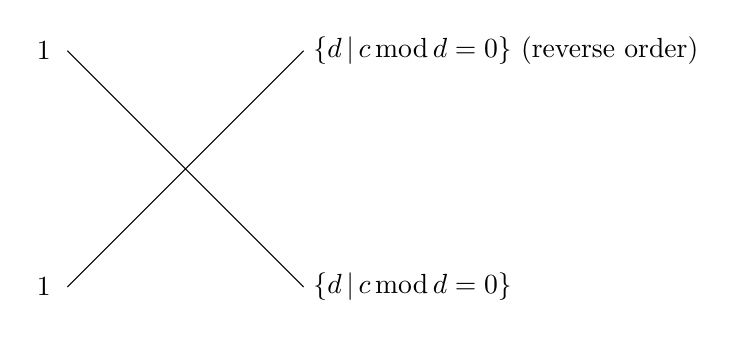
\begin{tikzpicture}[domain=-1:4]
    \draw (0,0) -- (3,3) node [right] {$\{d\mkern3mu \vert\mkern3mu c\mkern3mu \text{mod}\mkern3mu d = 0\}$ (reverse order)};
    \draw (0,3) -- (3,0) node [right] {$\{d\mkern3mu \vert\mkern3mu c\mkern3mu \text{mod}\mkern3mu d = 0\}$};
    \draw (-0.3, 3) node {$1$};
    \draw (-0.3, 0) node {$1$};

\end{tikzpicture} \\

Multiply this first diagonal like $1*d_r$ \\


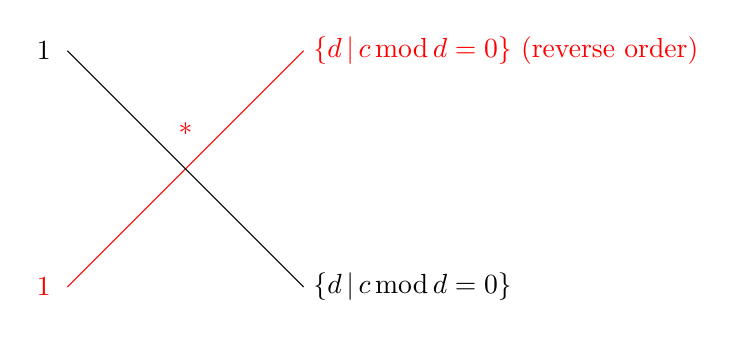
\begin{tikzpicture}[domain=-1:4]
    \draw[color=red] (0,0) -- (3,3) node [right] {$\{d\mkern3mu \vert\mkern3mu c\mkern3mu \text{mod}\mkern3mu d = 0\}$ (reverse order)};
    \draw (0,3) -- (3,0) node [right] {$\{d\mkern3mu \vert\mkern3mu c\mkern3mu \text{mod}\mkern3mu d = 0\}$};
    \draw (-0.3, 3) node {$1$};
    \draw[color=red] (-0.3, 0) node {$1$};
    \draw[color=red] (1.5, 2) node {$*$};
\end{tikzpicture} \\

Add the second diagonal by the vertical: \\

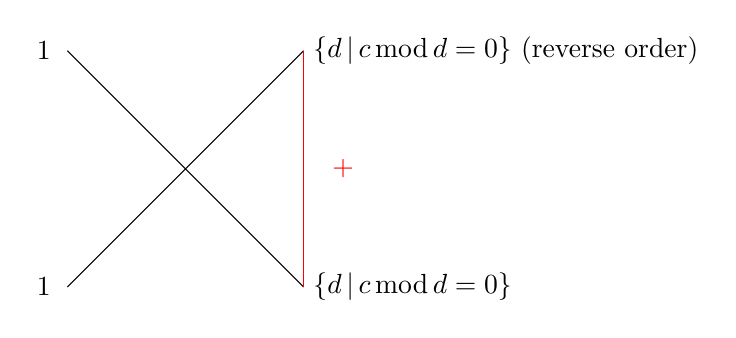
\begin{tikzpicture}[domain=-1:4]
    \draw (0,0) -- (3,3) node [right] {$\{d\mkern3mu \vert\mkern3mu c\mkern3mu \text{mod}\mkern3mu d = 0\}$ (reverse order)};
    \draw (0,3) -- (3,0) node [right] {$\{d\mkern3mu \vert\mkern3mu c\mkern3mu \text{mod}\mkern3mu d = 0\}$};
    \draw[color=red] (3,3) -- (3,0);
    \draw (-0.3, 3) node {$1$};
    \draw (-0.3, 0) node {$1$};
    \draw[color=red] (3.5, 1.5) node {$+$};

\end{tikzpicture} \\

And multiply again with $1*\frac{c}{d_r}$

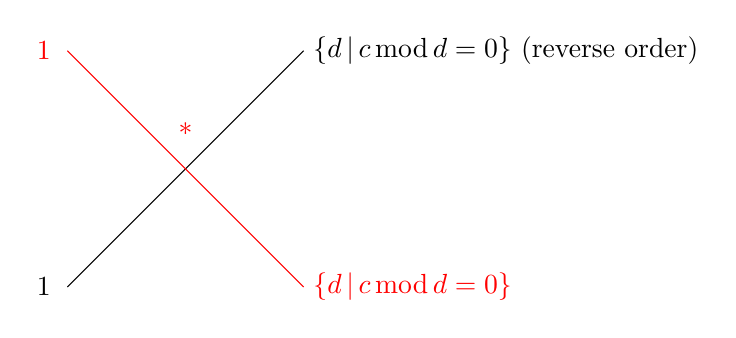
\begin{tikzpicture}[domain=-1:4]
    \draw (0,0) -- (3,3) node [right] {$\{d\mkern3mu \vert\mkern3mu c\mkern3mu \text{mod}\mkern3mu d = 0\}$ (reverse order)};
    \draw[color=red] (0,3) -- (3,0) node [right] {$\{d\mkern3mu \vert\mkern3mu c\mkern3mu \text{mod}\mkern3mu d = 0\}$};
    \draw[color=red] (-0.3, 3) node {$1$};
    \draw (-0.3, 0) node {$1$};
    \draw[color=red] (1.5, 2) node {$*$};

\end{tikzpicture}

At the end you get: 
$$
1*d_r+1*\frac{c}{d_r}
$$

If $a \neq 1$ then simply change the left hand side to include $\{d\mkern3mu \vert\mkern3mu a\mkern3mu \text{mod}\mkern3mu d = 0\}$. \\

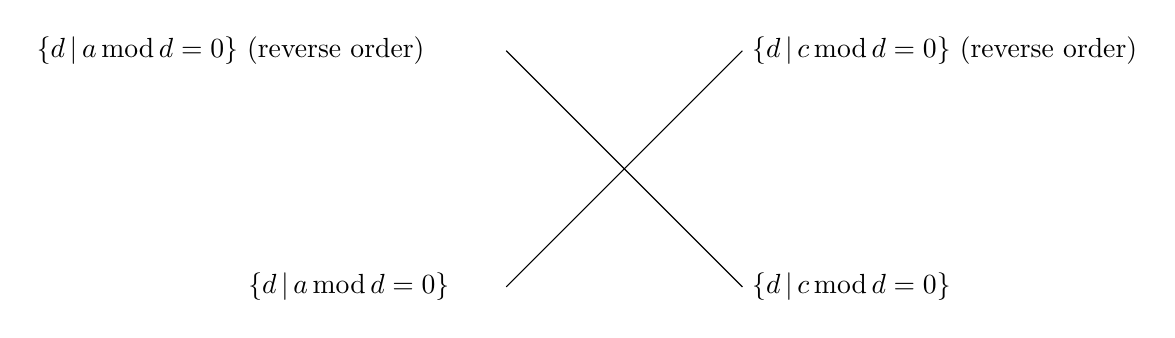
\begin{tikzpicture}[domain=-1:4]
    \draw (0,0) -- (3,3) node [right] {$\{d\mkern3mu \vert\mkern3mu c\mkern3mu \text{mod}\mkern3mu d = 0\}$ (reverse order)};
    \draw (0,3) -- (3,0) node [right] {$\{d\mkern3mu \vert\mkern3mu c\mkern3mu \text{mod}\mkern3mu d = 0\}$};
    \draw (-3.5, 3) node {$\{d\mkern3mu \vert\mkern3mu a\mkern3mu \text{mod}\mkern3mu d = 0\}$ (reverse order)};
    \draw (-2, 0) node {$\{d\mkern3mu \vert\mkern3mu a\mkern3mu \text{mod}\mkern3mu d = 0\}$};

\end{tikzpicture} \\

Note that: 
\begin{itemize}
    \item if $c > 0$ then dependent on whether $b > 0$ or $b < 0$ pick the positive or negative factors in $d$.
    \item otherwise, one of the factors in $d$ will be negative and the other chosen factor should be positive.
\end{itemize}

\subsubsection{Example}

$$
f(x)=3x^2-27x+60 \Longrightarrow f(x)=3(x^2-9x+20)
$$

Since $c > 0$ and $b < 0$, then both sets have to be negative for the equation to be true.

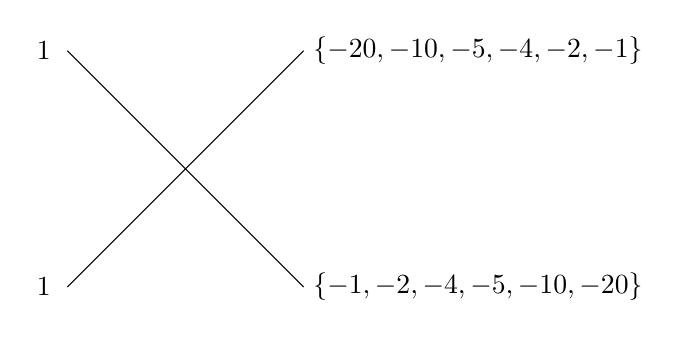
\begin{tikzpicture}[domain=-1:4]
    \draw (0,0) -- (3,3) node [right] {$\{-20, -10, -5, -4, -2, -1\}$};
    \draw (0,3) -- (3,0) node [right] {$\{-1, -2, -4, -5,-10, -20\}$};
    \draw (-0.3, 3) node {$1$};
    \draw (-0.3, 0) node {$1$};
\end{tikzpicture} \\

$$
1*\mathbf{-4}+1*\mathbf{-5}=-9
$$

Therefore:
$$
f(x)=3(x-4)(x-5)
$$

Since $a$ doesn't have to be $1$, this method scales well with more difficult quadratics. 

% i don't think this method makes sense

\section{Sets}


On the SAT, you may be given a set visually or in numbers. For this guide, we will use sets in this format:

$$
\{a_1, a_2, ... a_n\}
$$

\subsection{Domain and Range}

Domain is the total distance of the inputs. For the above set, the domain could be denoted as $n-1$ or $[1, n]$ because the first element is $a_1$ and the last is $a_n$.

The range is the total distance, which would be $\text{max}(\{a_1, a_2, ... a_n\}) - \text{min}(\{a_1, a_2, ... a_n\})$.

\subsection{Standard Deviation}

Standard deviation measures the total difference between the mean and each value in the set. 

$$
\sigma=\sqrt{\frac{1}{n}\sum_{i=1}^n(x_i-\mu)^2}
$$

Where $n$ is the length, $x_i$ is each item in the set, and $\mu$ is the mean. \\
The SAT tests whether you can conceptually understand the deviation or not. So if your data typically is further from the mean, it has a higher standard deviation. Note that spread is unrelated to the range. Don't let outliers in the range confuse you.

Typically, on the SAT they will look like: \\

\begin{tikzpicture}
    \draw (0,0) -- (4,0);

    \draw (0,-0.25) -- (0,0.25);
    \draw (0, -0.5) node {$1$};

    \draw (1,-0.25) -- (1,0.25);
    \draw (1, -0.5) node {$2$};

    \draw (2,-0.25) -- (2,0.25);
    \draw (2, -0.5) node {$3$};

    \draw (3,-0.25) -- (3,0.25);
    \draw (3, -0.5) node {$4$};

    \draw (4,-0.25) -- (4,0.25);
    \draw (4, -0.5) node {$5$};

    \fill (0,0.5) circle (2pt);
    \fill (0,1) circle (2pt);
    \fill (2,0.5) circle (2pt);
    \fill (3,0.5) circle (2pt);
    \fill (3,1) circle (2pt);
    \fill (3,1.5) circle (2pt);

    \draw (2,-1) node {Set $A$};

    \draw (5,0) -- (9,0);

    \draw (5,-0.25) -- (5,0.25);
    \draw (5, -0.5) node {$1$};

    \draw (6,-0.25) -- (6,0.25);
    \draw (6, -0.5) node {$2$};

    \draw (7,-0.25) -- (7,0.25);
    \draw (7, -0.5) node {$3$};

    \draw (8,-0.25) -- (8,0.25);
    \draw (8, -0.5) node {$4$};

    \draw (9,-0.25) -- (9,0.25);
    \draw (9, -0.5) node {$5$};

    \fill (6,0.5) circle (2pt);
    \fill (6,1) circle (2pt);
    \fill (7,0.5) circle (2pt);
    \fill (8,0.5) circle (2pt);
    \fill (9,0.5) circle (2pt);
    \fill (9,1) circle (2pt);

    \draw (7,-1) node {Set $B$};
\end{tikzpicture}

Set $B$ has the smaller standard deviation.


%\section{Word Problems}
%
%You can't really predict what these will be. For 

\section{Trigonometry}

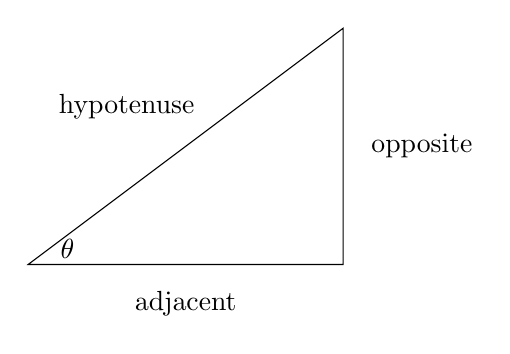
\begin{tikzpicture}
    \draw (0,0) -- (4,0) -- (4,3) -- cycle;
    \draw (0.5,0.2) node {$\theta$};
    \draw (2, -0.5) node {adjacent};
    \draw (1.25, 2) node {hypotenuse};
    \draw (5, 1.5) node {opposite};
\end{tikzpicture}

$$
\sin(\theta) = \frac{\text{opposite}}{\text{hypotenuse}}
$$
$$
\cos(\theta) = \frac{\text{adjacent}}{\text{hypotenuse}}
$$
$$
\tan(\theta) = \frac{\text{opposite}}{\text{adjacent}}
$$


\end{document}
